\chapter{Contesto smart city}
\label{cha:smartcity}

Nel seguente capitolo verrà introdotto il concetto di \textit{smart city} con una particolare approfondimento alla \textit{smart mobility}. Ho deciso di presentare questo argomento poiché il bot è considerabile un servizio interno a questo ambito. Inoltre, verranno analizzate le principali applicazioni utilizzate nelle città più smart del mondo.

Innanzitutto, con il termine \textit{smart city} definiamo una città che gestisce le risorse in modo intelligente, che mira a diventare economicamente sostenibile ed energeticamente autosufficiente, ed è attenta alla qualità della vita e ai bisogni dei propri cittadini\cite{SmarCity}.

\section{Smart mobility}
\label{sec:smart-mobility}

La \textit{Smart Mobility} è uno strumento utile ad ottenere lo sviluppo sostenibile delle città. Il termine fa riferimento a: tecnologia, infrastrutture per la mobilità (parcheggi, reti di ricarica, segnaletica, veicoli), soluzioni per la mobilità (tra cui i modelli di \textit{new mobility}) e persone. Tra i principali obiettivi da raggiungere, grazie all'introduzione di queste novità, troviamo: la riduzione del traffico e dell'inquinamento, la creazione di flussi intelligenti e senza interruzioni e il rafforzamento delle economie di scala per la promozione di una mobilità che sia accessibile a tutti. \cite{SmartMobility}\\

\noindent La\textit{ Smart mobility}, fenomeno ampio e complesso, è basato sui seguenti principi:

\begin{enumerate}
    \item  \textit{Flessibilità}: grazie alle molteplici modalità di trasporto chi si sposta ha la possibilità di scegliere quale di queste è la migliore in base al contesto;
    \item  \textit{Efficienza}: permette al viaggiatore di arrivare a destinazione con il minimo sforzo e nel più breve tempo possibile;
    \item  \textit{Integrazione}: il tragitto completo viene pianificato integrando tutti i mezzi disponibili;
    \item \textit{Tecnologie pulite}: lo spostamento dai veicoli inquinanti a quelli a zero emissioni;
    \item \textit{Sicurezza}: drastica riduzione di morti e feriti; 
    \item \textit{Accessibilità}: la \textit{smart mobility} deve poter essere accessibile a tutti, in tutte le sue forme;
    \item \textit{Benefici sociali}: la \textit{smart mobility} deve aiutare a migliorare la qualità della vita. 
\end{enumerate}

\subsection{Esempi}

\subsubsection{Smart parking}

\begin{wrapfigure}{r}{0.4\textwidth}
\centering
\frame{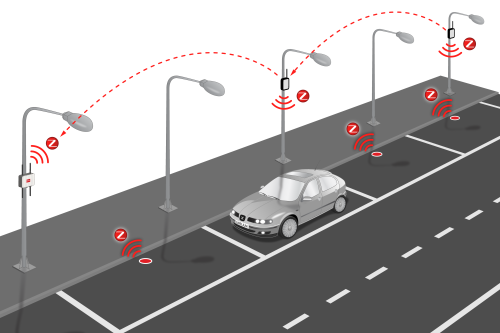
\includegraphics[scale=0.7]{smart-parking.png}}
\caption{Smart parking}
\label{fig:smart_parking}
\end{wrapfigure}

Secondo alcune statistiche, il 40\% del traffico nelle aree urbane è provocato dai guidatori che stanno cercando parcheggio, causando congestione, rumore e inquinamento. Barcellona, ad esempio, per migliorare questa situazione ha adottato la tecnologia dei parcheggi intelligenti. Nelle strade, è stato installato un sistema di sensori che comunicano ai cittadini, tramite applicazioni e dispositivi mobili, la condizione dei posti auto disponibili. Utilizzando display e \textit{embeddando} sensori nelle aree \textit{free parking}, uniti ad app che consentono la ricezione delle informazioni e la gestione dei pagamenti, Barcellona è riuscita a rendere più fluido il traffico, ridurre il tempo e il carburante richiesto, portando benefici anche all'ambiente.  

Tra i servizi di \textit{smart parking} troviamo, ad esempio, il \textit{“community-based parking”}: dei veicoli connessi tra loro con un hardware di connettività identificano, attraverso dei sensori, gli spazi disponibili mentre passano. Ciò permette agli automobilisti, in cerca di parcheggio, di beneficiare di questi dati acquisiti dalla "comunità" e di essere guidati sul posto con informazioni in tempo reale. 

\subsubsection{Semafori intelligenti}

In Olanda, sull’autostrada N205 a Noord-Holland, vicino ad Amsterdam, sono presenti dei semafori in grado di "parlare" in tempo reale, attraverso un'applicazione, con i viaggiatori. Le informazioni fornite riguardano le condizioni del traffico e permettono di dare priorità a determinati gruppi di automobilisti. Inoltre, già a partire dal 2016, sono stati installati, nella città di 's-Hertogenbosch, dei semafori smart in grado di regolare la durata del verde in base alle esigenze del traffico. Quando, ad esempio, i semafori registrano una maggiore affluenza di biciclette, automobili o mezzi di trasporto pubblico prolungano il via libera, così da non creare ingorghi. 

\subsubsection{Mobility as a Service (MaaS)}

\begin{wrapfigure}{r}{0.4\textwidth}
\centering
\frame{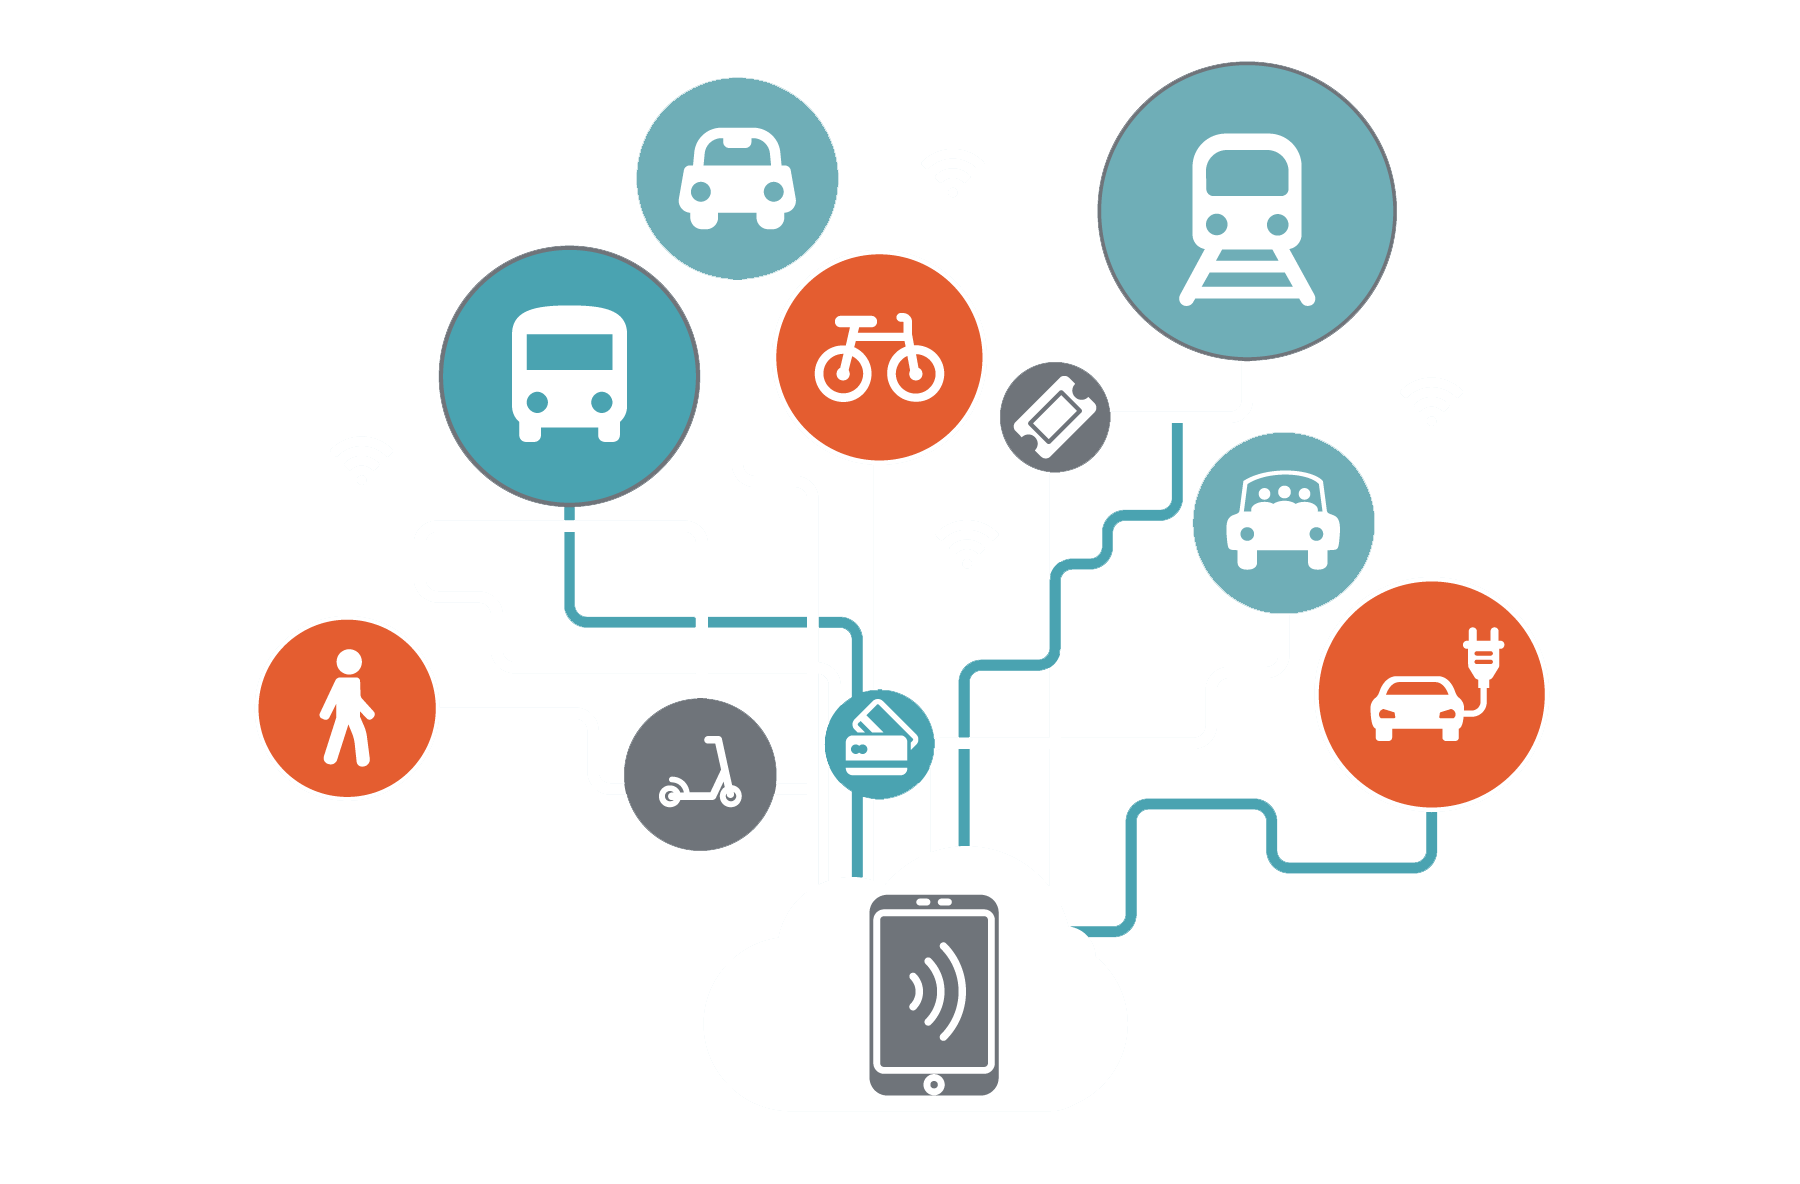
\includegraphics[scale=0.095]{maas.png}}
\caption{MaaS app}
\label{fig:maas}
\end{wrapfigure}

Il \textit{MaaS} (Mobility as a Service) rappresenta un nuovo modello di business per l'erogazione di servizi di trasporto. Come tutti i modelli \textit{"as a service"}, prevede un abbonamento mensile a regime forfait che assicura l'utilizzo personalizzato di un \textit{bundle} di trasporti pubblici e privati, che siano treni, bus, taxi, car o bike sharing, in modo illimitato con un unico abbonamento (\textit{all in one}), tendenzialmente attraverso un'app. 

L’Autorità del Trasporto regionale di Helsinki consente l’accesso ai dati relativi a percorsi, orari e costi attraverso le API aperte. L’app è inoltre integrata con i calendari degli utenti in modo che questi possano programmare in anticipo il proprio viaggio e scegliere in base a criteri come velocità, prezzo e comfort.

\section{Competitor}
\label{sec:competitor}

Dopo aver approfondito il concetto di \textit{smart mobility} è importante fare un'analisi dei potenziali servizi competitor. Questo permette di stabilire cosa manca nel mercato attuale e conoscere le preferenze degli utenti, oltre a rendere più chiaro in che direzione sarà possibile sviluppare il bot Telegram.

\subsection{Bot telegram}
Innanzitutto, sono partito ricercando dei bot telegram legati alla mobilità. La ricerca non è stata banale dato che non esiste un sistema centrale, come può essere ad esempio il \textit{Play Store} per le applicazioni mobile Android, che raccoglie e categorizza i bot esistenti e verifica il loro stato. Quindi, i bot sono stati ricercati tramite \textit{Google} e tramite \textit{BotsArchive}, un sito web che tramite segnalazione degli utenti o sviluppatori raccoglie i bot Telegram e permette agli utenti di votare i migliori. Sfortunatamente, molti di questi risultavano offline e non è stato quindi possibile testarli ed inserirli in questo approfondimento, sebbene sembrassero molto validi.

\subsubsection{ViaggiaTrentoBot}

\textit{ViaggiaTrentoBot} supporta la mobilità urbana sostenibile di Trento. Esso permette di consultare gli orari degli autobus urbani di Trento e dei treni delle ferrovie Brennero, Valsugana e Trento-Mezzana. Inoltre, permette di controllare in diretta i posti liberi nei parcheggi e la disponibilità di biciclette nei punti di bike sharing della città. L'interfaccia è abbastanza intuitiva ma, sfortunatamente, è limitato alla sola città di Trento e non fornisce informazioni sulla posizione dei mezzi in tempo reale.

\subsubsection{GTT Orari degli arrrivi in fermata}
Questo bot consente di conoscere gli arrivi previsti alla fermata dei tram e dei bus urbani e suburbani di Torino e di visualizzare le rivendite autorizzate di biglietti più vicine. Per le ricerche è sufficiente inserire il numero o il nome della fermata di interesse; a questo punto si riceverà un messaggio con gli orari dei passaggi in tempo reale ed una mappa in cui è mostrata la posizione della fermata e la zona circostante. L'interfaccia di questo bot è confusionaria ed è difficile da utilizzare senza essere guidati.

\subsubsection{TrenItBot}

TrenItBot è un bot di Telegram che ti permette di cercare e seguire i treni italiani mostrandoti orari, ritardi, binari, fermate, cancellazioni e scioperi in tempo reale. Se si conosce il numero del treno che si vuole seguire, si può inviare il comando \textit{/segui}. Altrimenti, usando il comando \textit{/cerca} è possibile trovare una soluzione di viaggio se si conosce la stazione di origine, quella di destinazione, e l'orario (approssimato) di partenza. Il bot è molto intuitivo anche per utenti al primo utilizzo ed è, secondo me, il migliore provato di questa categoria.

\subsubsection{Altri bot}
Quasi tutti i bot Telegram legati alla mobilità di città non italiane erano offline, in particolare ho trovato dei bot per le città di Dublino e Madrid. L'unico funzionante che ho trovato è \textit{Bus Eta Bot}. Questo permette di conoscere, in tempo reale, il tempo di arrivo previsto degli autobus di Singapore e fornisce altre informazioni sull'autobus in arrivo come il tipo di autobus, l'affluenza e se è accessibile o meno in sedia a rotelle.

\begin{figure}[htb]
    \centering 
\begin{subfigure}{0.20\textwidth}
\frame{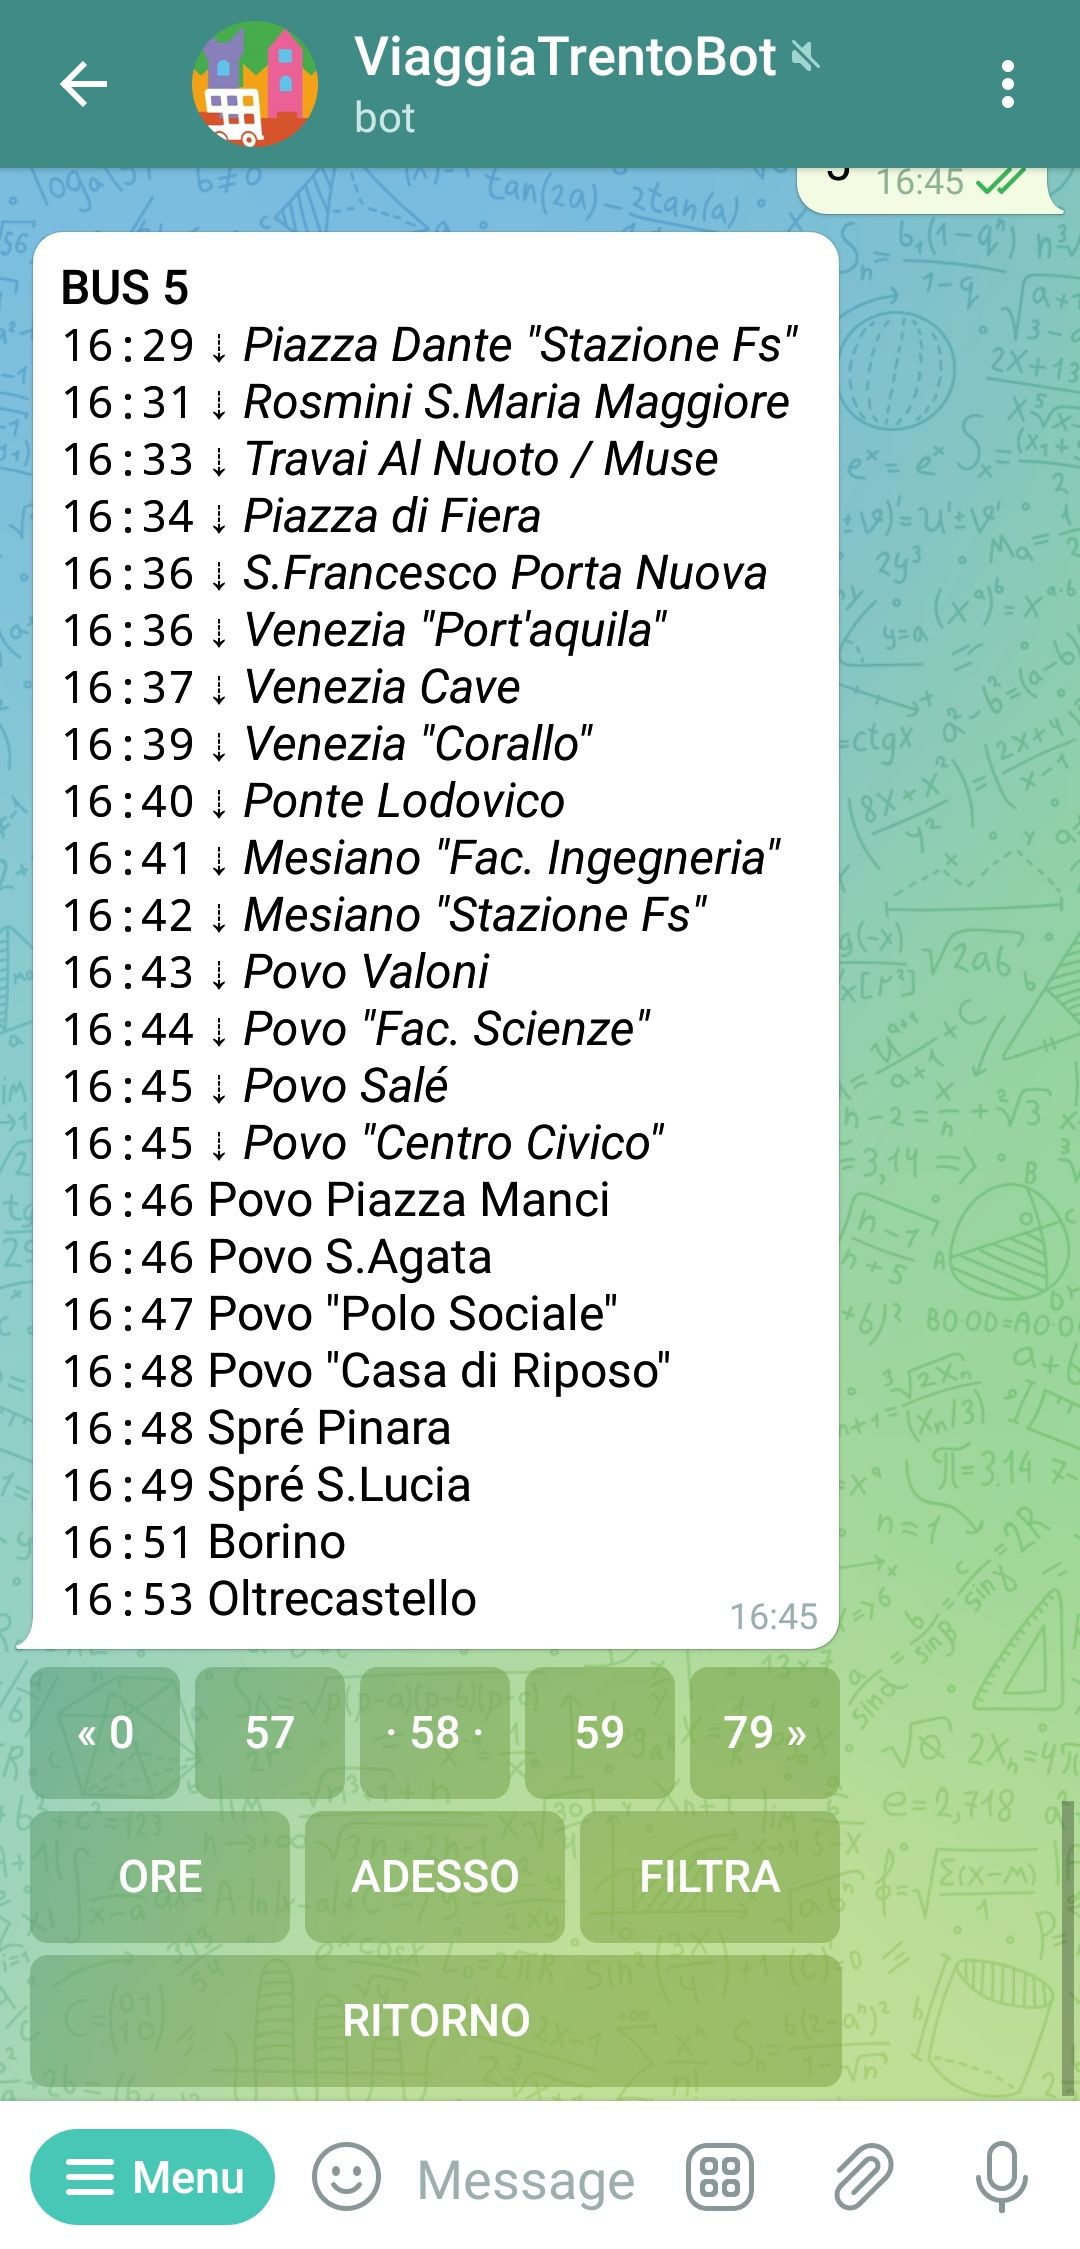
\includegraphics[width=\linewidth]{competitor_viaggiatrento.jpg}}
\caption{ViaggiaTrentoBot}
\label{fig:viaggia_trento}
\end{subfigure}\hfil
\begin{subfigure}{0.20\textwidth}
\frame{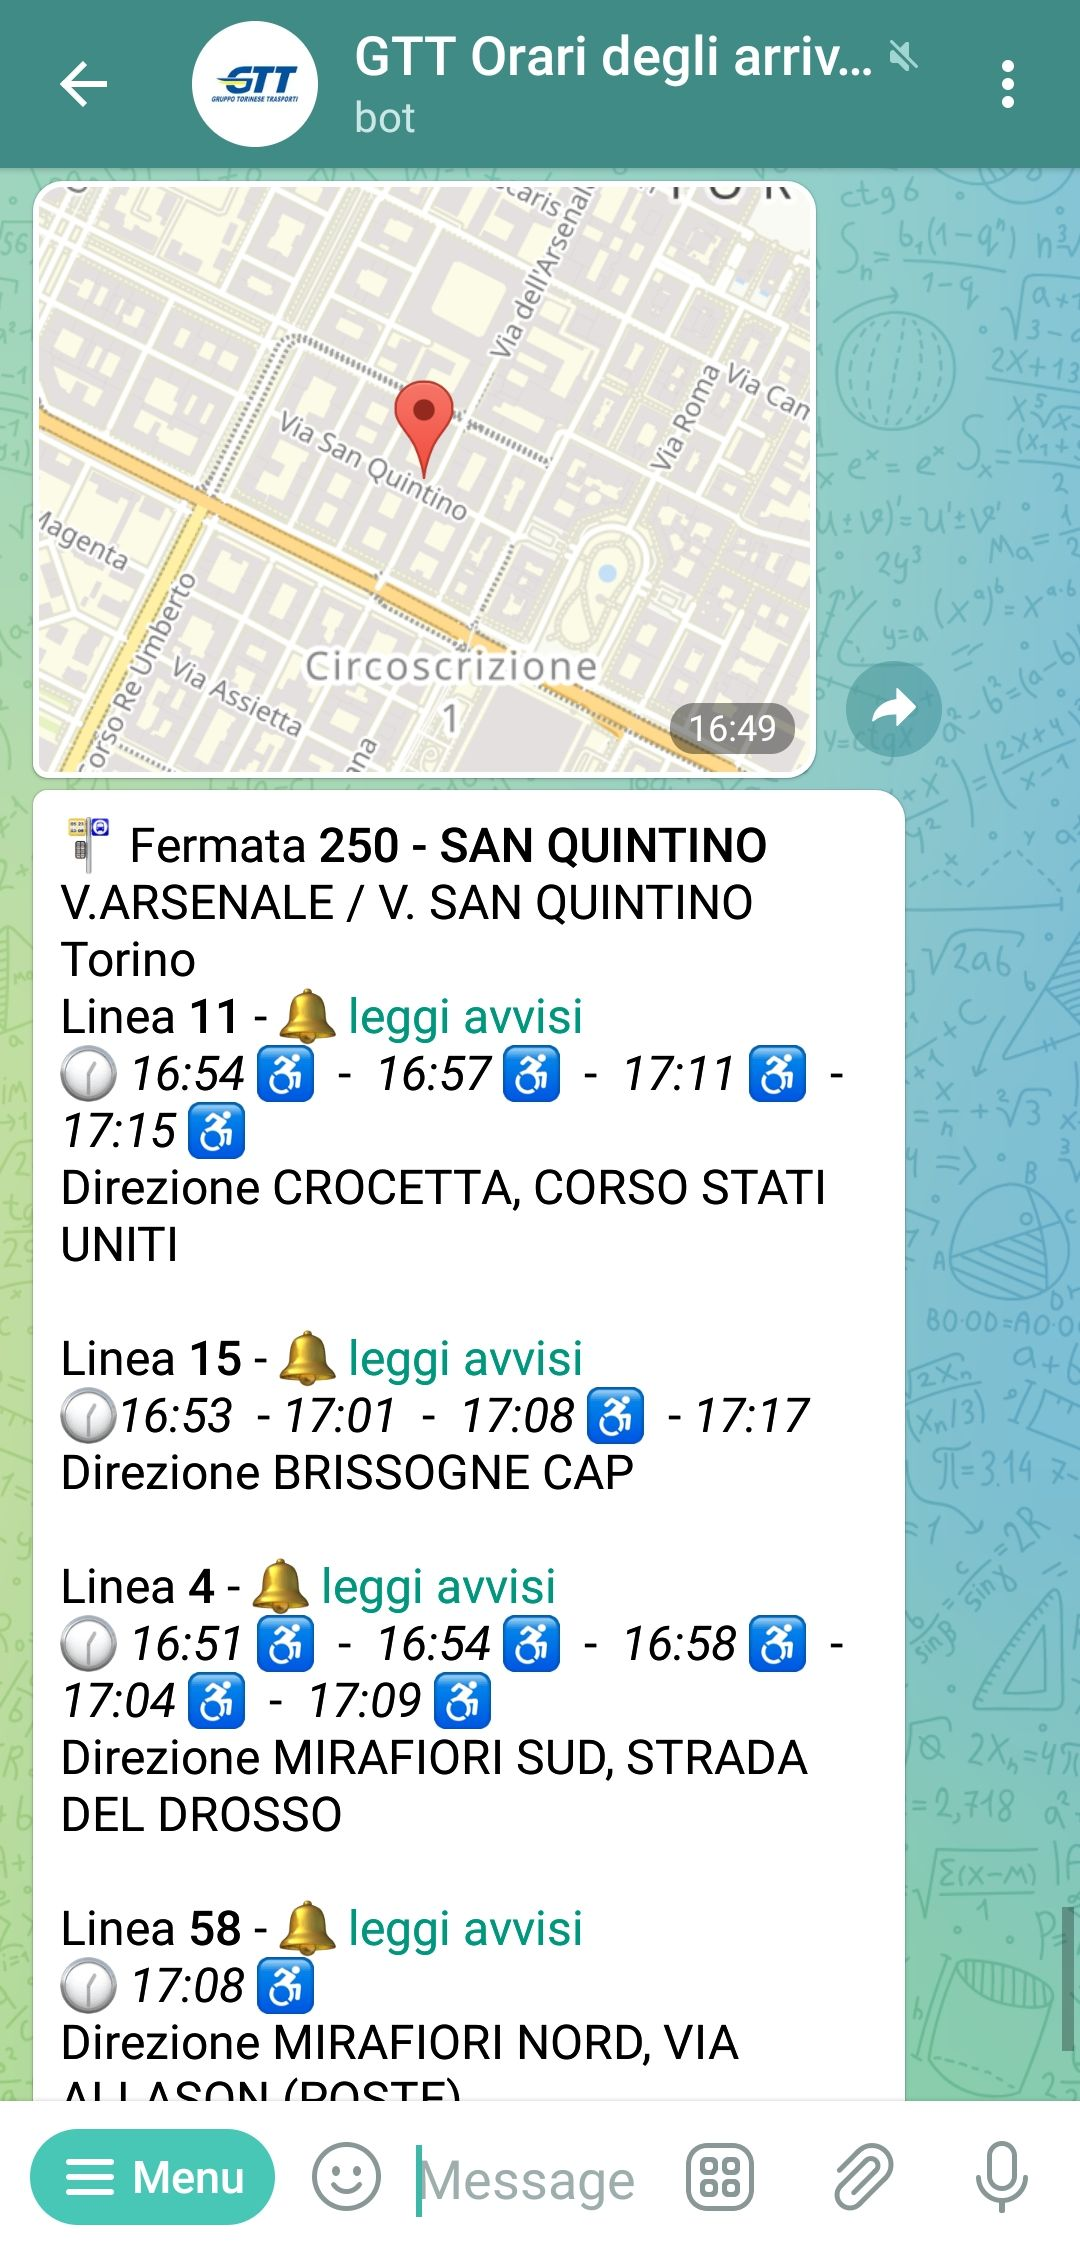
\includegraphics[width=\linewidth]{competitor_gtt.jpg}}
\caption{GTT Orari}
\label{fig:gtt_orari}
\end{subfigure}\hfil 
\begin{subfigure}{0.20\textwidth}
\frame{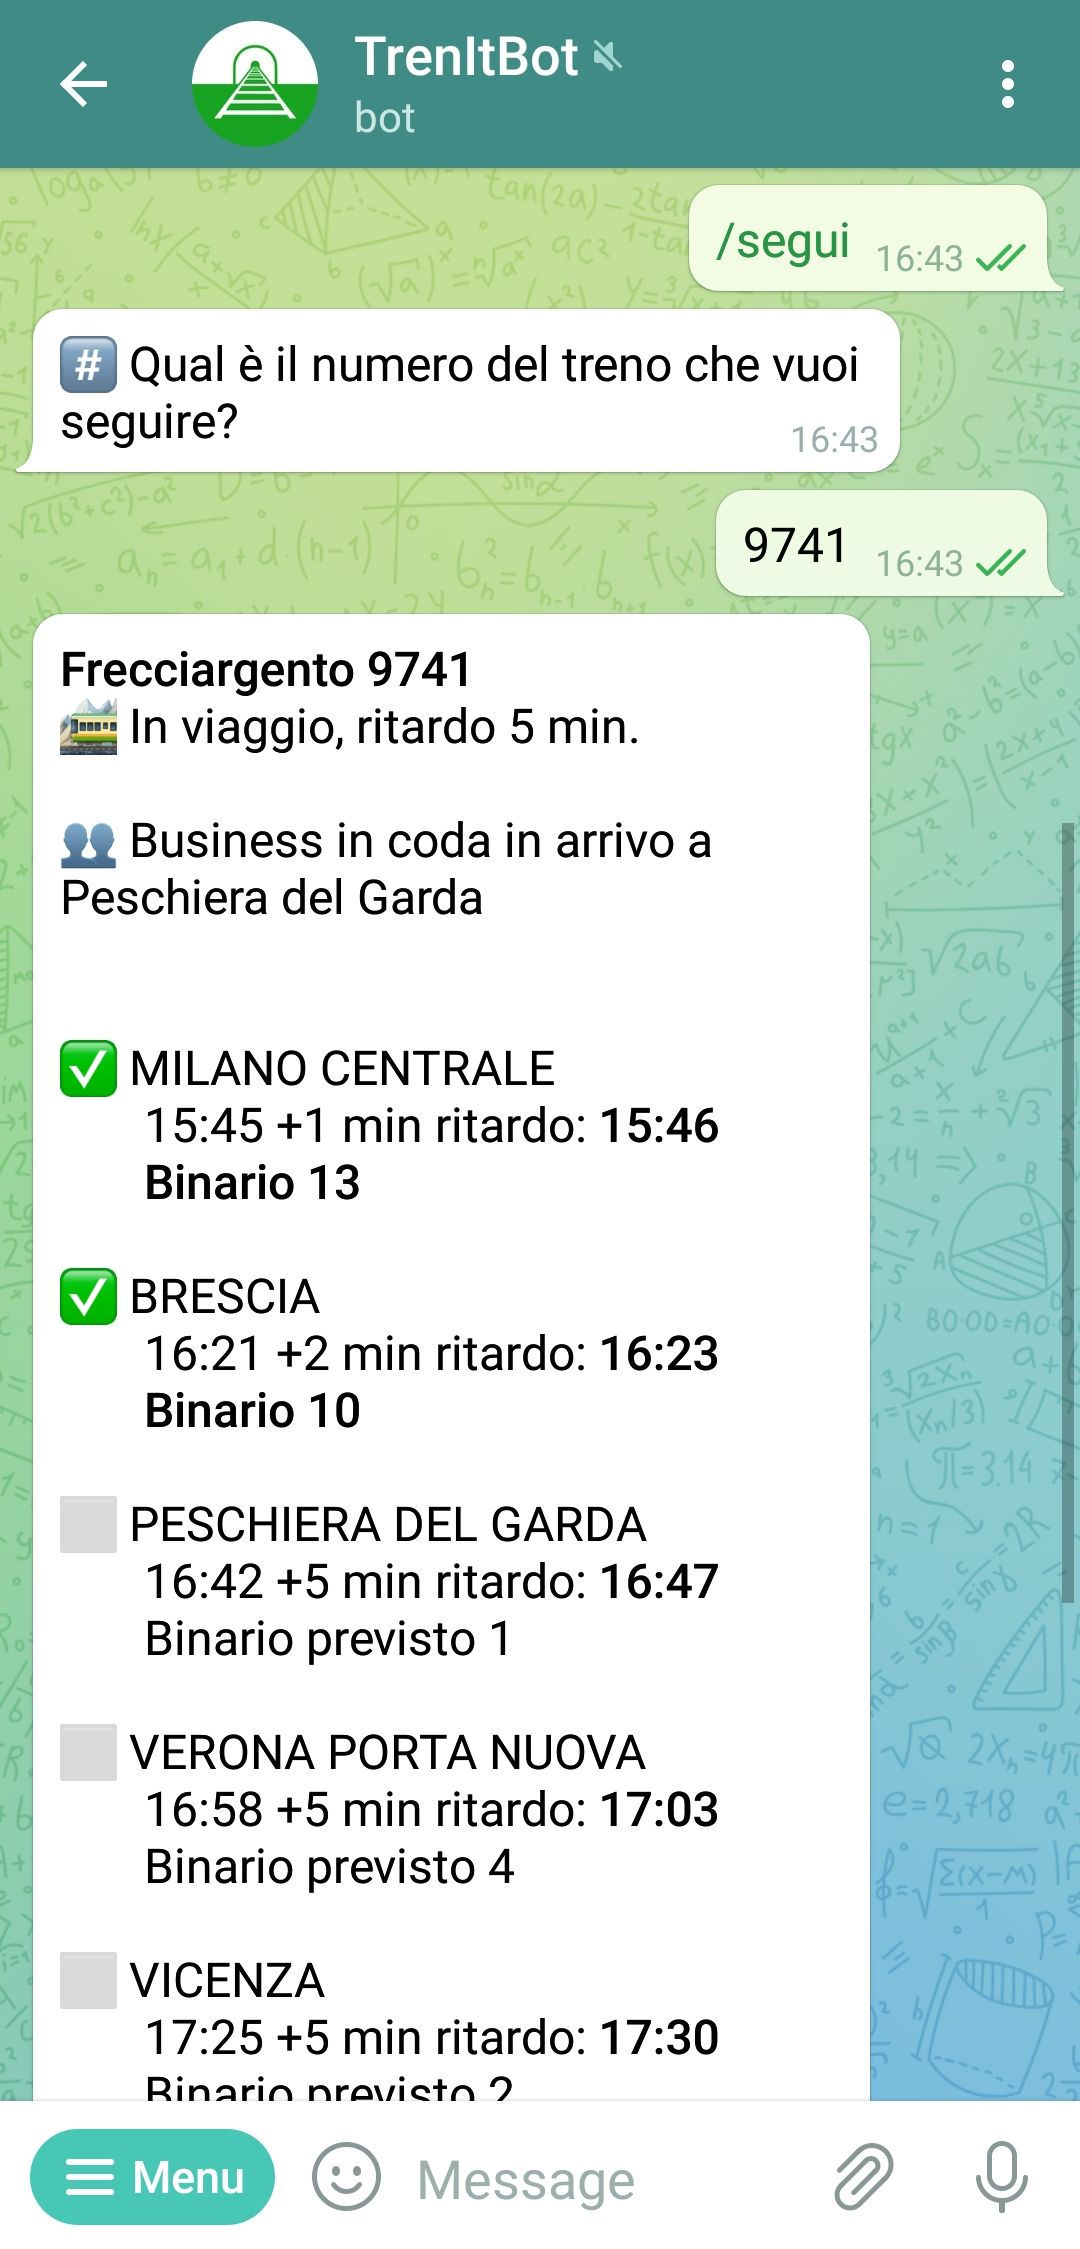
\includegraphics[width=\linewidth]{competitor_trenitbot.jpg}}
\caption{TrenItBot}
\label{fig:trenit_bot}
\end{subfigure}\hfil 
\begin{subfigure}{0.20\textwidth}
\frame{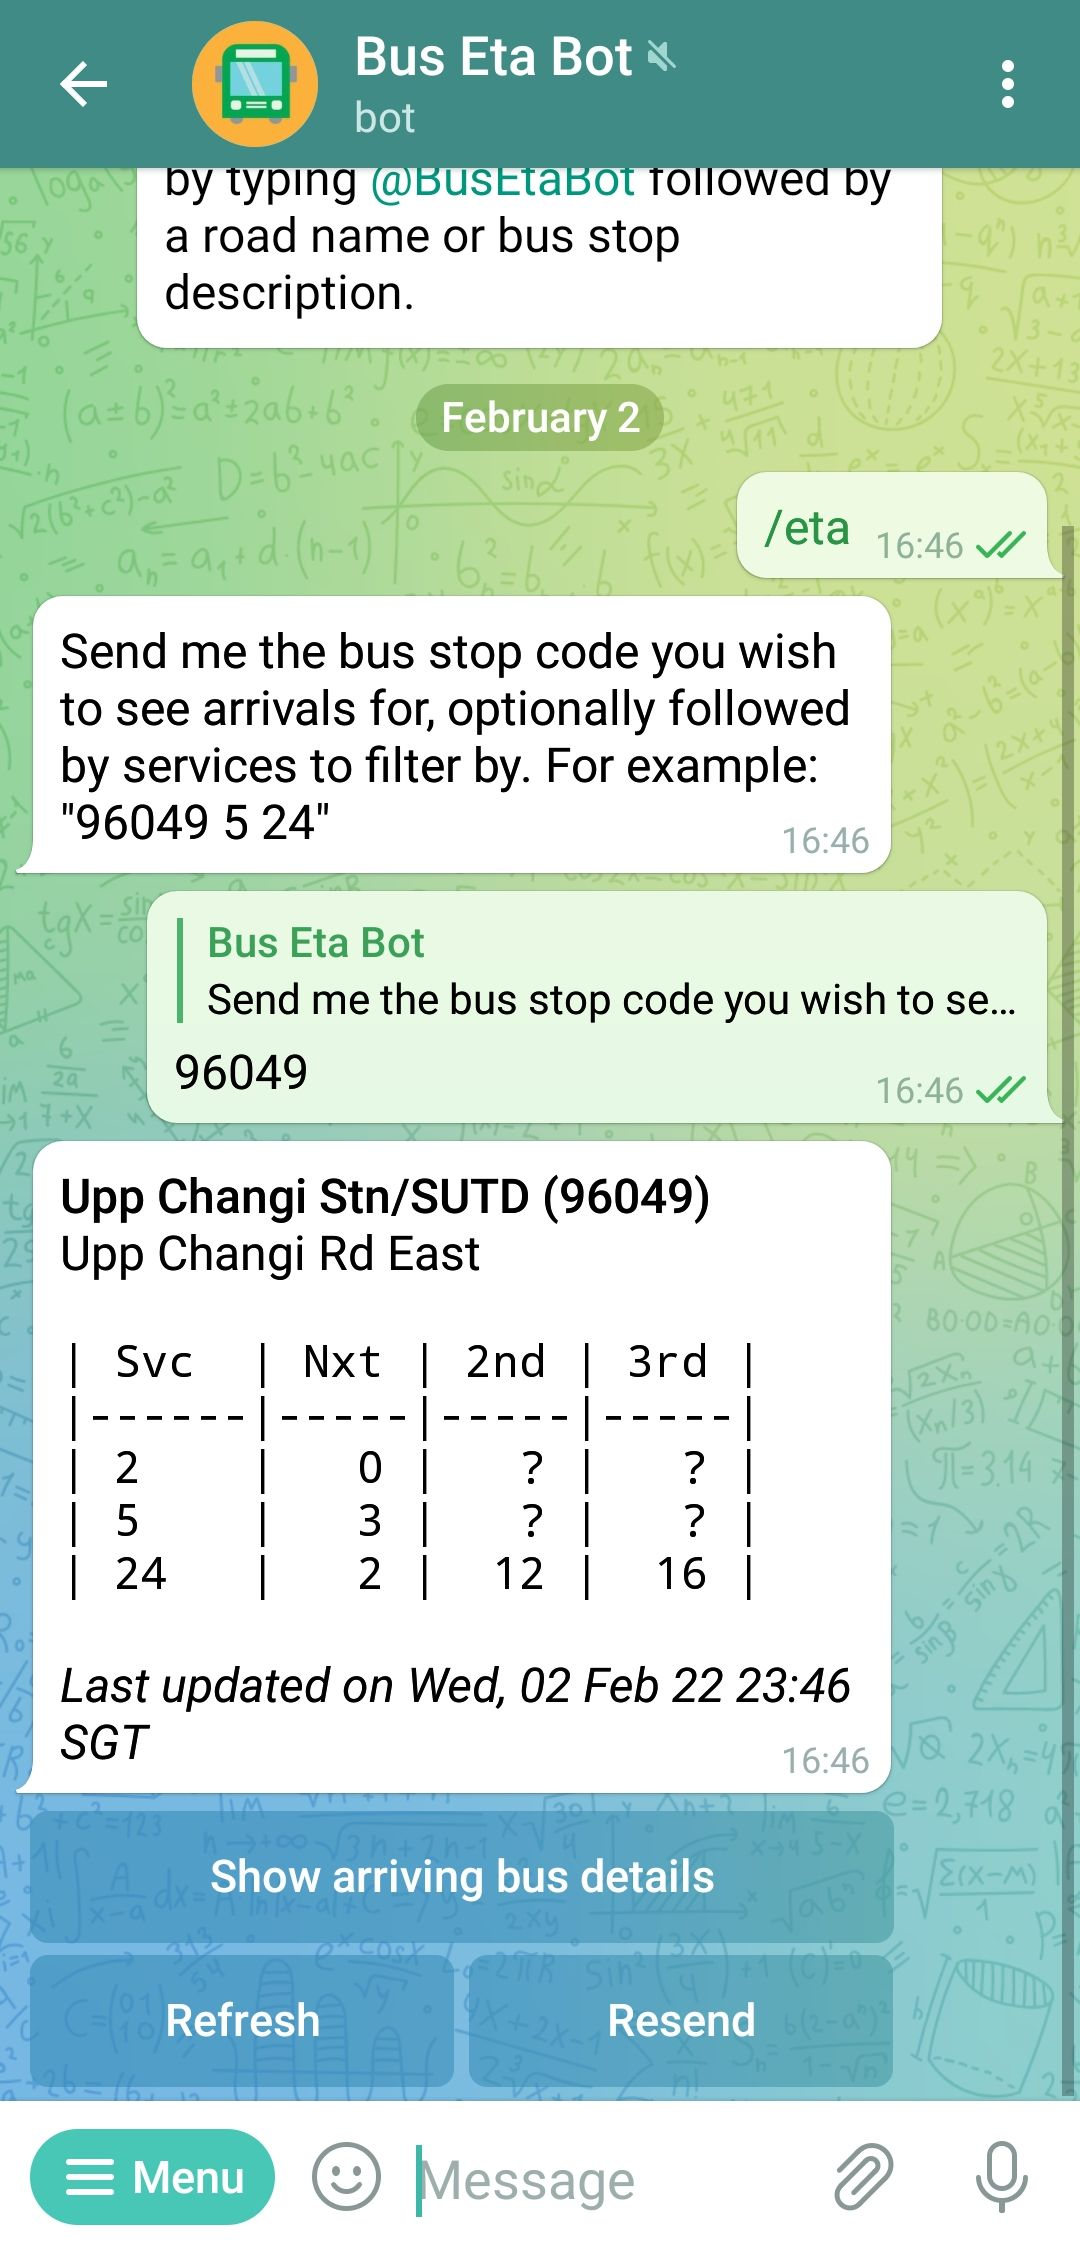
\includegraphics[width=\linewidth]{competitor_buseta.jpg}}
\caption{Bus Eta Bot}
\label{fig:bus_eta_bot}
\end{subfigure}
\caption{
\label{fig:bot_competitor}Bot telegram competitor}
\end{figure}

\subsection{Applicazioni mobile}
A differenza dei bot Telegram, non è stato difficile trovare applicazioni mobile legate alla \textit{smart mobility} operanti sia nel mondo che in Italia. Nonostante la diffusione di questi progetti a livello locale dia una grande spinta all’adozione di modelli di vita più sostenibili, sfortunatamente, non c’è ancora un servizio che possa essere utilizzato in tutta Italia, indipendentemente dalla regione e dalla città di residenza. Questo pone dei limiti, soprattutto per chi viaggia spesso all’interno dei confini nazionali. Di seguito ho deciso di riportare e descrivere brevemente tre applicazioni attualmente attive nel settore della \textit{smart mobility} che offrono dei servizi originali.

\newpage

\subsubsection{Moovit}

\begin{wrapfigure}{r}{0.50\textwidth}
\centering
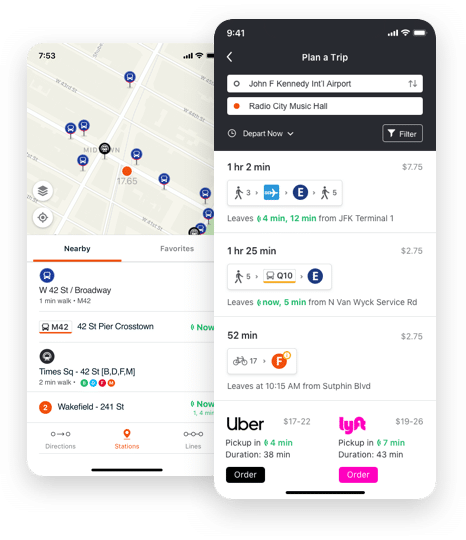
\includegraphics[scale=0.45]{app_moovit.png}
\caption{App Moovit}
\label{fig:app_moovit}
\end{wrapfigure}

 Questa azienda, leader mondiale di soluzioni di \textit{MaaS} (Mobility as a Service) e di \textit{journey planning}, ora proprietà di \textit{Intel}, nasce come start-up israeliana. L'app consente di pianificare e pagare un percorso, scegliendo il tragitto e il mezzo più conveniente, tutto attraverso lo smartphone. Ciò è reso possibile combinando dati ufficiali a \textit{crowdsourced data} (dati ottenuti dagli utenti attraverso la rete), questo permette di fornire informazioni in tempo reale sui servizi di trasporto pubblico. A questo si aggiungono i dati su taxi, Uber, Lyft, biciclette, monopattini, scooter e ciclomotori, car sharing e molto altro. Inoltre, l'app, attraverso notifiche push, informa gli utenti su variazioni al servizio di trasporto pubblico o allerte meteo. 
 Attualmente è disponibile in Italia solo nelle grandi città. Essa è in continuo aggiornamento, infatti, tra gli ultimi aggiornamenti pubblicati troviamo, ad esempio, i dati sull'affluenza dei singoli bus in tempo reale, tramite la segnalazione degli utenti. 
 Esistono molte app simili come ad esempio Transit e Citymapper, ma Moovit è la più completa nel suo genere.

\subsubsection{EasyPark}

\begin{wrapfigure}{r}{0.55\textwidth}
    \centering 
\begin{subfigure}{0.23\textwidth}
\centering
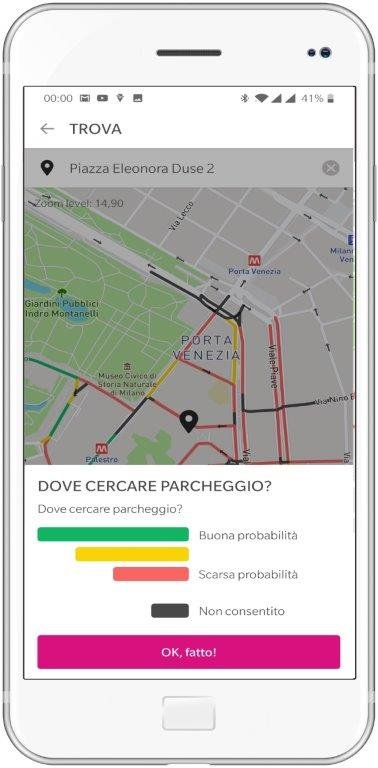
\includegraphics[scale=0.55]{app_easypark.jpg}
\caption{Ricerca parcheggio}
\label{fig:app_easypark_1}
\end{subfigure}\hfil
\begin{subfigure}{0.23\textwidth}
\centering
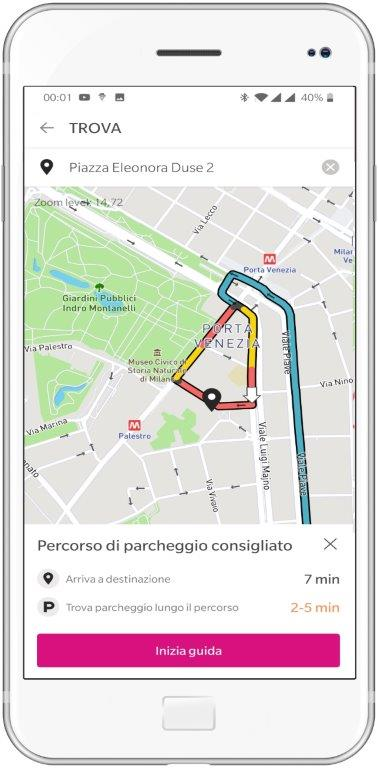
\includegraphics[scale=0.55]{app_easypark_2.jpg}
\caption{Percorso consigliato}
\label{fig:app_easypark_2}
\end{subfigure}
\caption{
\label{fig:app_easypark}App EasyPark}
\end{wrapfigure}

Questa app offre una visione completa delle diverse soluzioni di sosta, di breve o lunga durata, comprese di prezzi e distanza dalla destinazione prescelta. All'interno dell'app troviamo diversi servizi:
\begin{itemize}
    \item \textit{parking planner}, che permette la prenotazione del parcheggio in anticipo;
    \item \textit{parking guidance}, che aiuta a trovare posti auto disponibili nella città;
    \item  \textit{find park}, strumento che fornisce il percorso ottimale per trovare parcheggi su strada o garage disponibili vicino ad un luogo d'interesse, unito ad una mappa in cui i colori delle vie chiariscono la probabilità di trovare parcheggio (Vedi figura \ref{fig:app_easypark}\subref{fig:app_easypark_1}).
\end{itemize} 


\noindent Inoltre, è possibile gestire la sessione di sosta in base alle proprie necessità, pagando, attraverso diverse modalità, solo il tempo d'uso effettivo senza rischio di multe o bisogno di parchimetri. 

\subsubsection{BusLive}

Questa app, meno conosciuta delle precedenti, permette di visualizzare la posizione GPS dei mezzi di trasporto pubblico. Questo permette di pianificare i trasferimenti tenendo conto della reale situazione del traffico e scegliendo il veicolo che permette di arrivare nel luogo selezionato nel minor tempo possibile.
Nonostante l'idea di base sia molto buona, l'interfaccia utente e il design potrebbero essere maggiormente curati. 
Questo servizio è disponibile solo in due città italiane, Roma e Torino, e in alcune città della Polonia.

\subsection{In Trentino}

Oltre al bot precedentemente citato, a livello trentino, troviamo altre app legate alla \textit{smart mobility} locale. In particolare: 
\begin{itemize}
    \item \textit{Muoversi in Trentino}, che fornisce informazioni georeferenziate in tempo reale sui servizi di trasporto pubblico relativamente a corse/linee, orari, tempi di percorrenza, eventuali ritardi dei mezzi pubblici, funzioni di “trova percorso”, integrazione con i servizi di bike sharing;
    \item \textit{OpenMove}, permette l'acquisto e la convalida di biglietti singoli, di gruppo o abbonamenti, cercare i percorsi e orari dei mezzi provinciali;
    \item \textit{trentinotrasporti.it}, sito ufficiale del trasporto pubblico trentino, oltre alla ricerca di percorsi, consultazione degli orari in pdf e di tutte le informazioni necessarie, permette di vedere in tempo reale la posizione dei treni della ferrovia Trento-Mezzana con l'orario di arrivo nelle diverse stazioni. 
\end{itemize}
